\documentclass[11pt]{article}
\usepackage[left=3.5cm,right=3.5cm,top=2.5cm,bottom=2.5cm]{geometry}
%\usepackage[spanish]{babel}
\overfullrule = 5mm

\usepackage{amsmath,amsfonts,amsthm}
\usepackage{enumitem,mathtools,graphicx}
\setenumerate[0]{label=(\alph*)}

\newtheorem{definition}{Definición}
\newtheorem{reminder}{Recordatorio}
\newtheorem{exercise}{Ejercicio}
\newtheorem*{sol}{Solución}
\newtheorem*{theorem}{Teorema}

\newcommand\fd{\mathrm{fd}}
\newcommand\N{\mathbb N}
\newcommand\R{\mathbb R}
\newcommand\C{\mathbb C}
\newcommand\ol\overline
\newcommand\<{\langle}
\renewcommand\>{\rangle}

%\usepackage{csquotes}
%\usepackage[style=authoryear]{biblatex}
%\addbibresource{references.bib}

\title{Análisis numérico para ecuaciones diferenciales \\
Examen parcial 3}
\author{Jorge Alfredo Álvarez Contreras}

\begin{document}
\maketitle

\section*{Ejercicios}

\begin{exercise}
  Considere el problema de valores en la frontera
  \begin{equation}
    \left\{
      \begin{aligned}
        &-u''(x) = \pi^{2}\sin(\pi x), \quad x\in(0,1),
        \\
        &u(0) = 0, \quad u(1)=0.
      \end{aligned}
    \right.
  \end{equation}
  Construya a mano el sistema de ecuaciones resultante de aproximar el
  problema mediante elementos finitos (usando las bases polinomiales
  de grado $1$) en la malla con nodos
  $0,\frac{1}{3},\frac{1}{2},\frac{3}{4},1$. Elabore una gráfica de
  $u$ vs $u_h$.
\end{exercise}
\begin{sol}
  Recordemos que el problema es
  \[
  \begin{aligned}
    &-u''(x) = f(x), \quad x\in(0,1),
    \\
    &u(0) = 0, \quad u(1)=0.
  \end{aligned}
  \]
  donde $f(x)=\pi^{2}\sin(\pi x)$.
  Sea $u$ es una solución del problema.
  Sea $V$ el espacio de funciones $v$ con derivada débil $v'\in L^{2}$
  y con $v(0)=v(1)=0$.
  Para cualquier $v\in V$, podemos multiplicar ambos lados de la
  ecuación $-u''=f$ e integrar en $[0,1]$. Usando integración por
  partes, obtenemos
  \begin{equation}
    \int_0^{1}u'v' = \int_0^{1} vf
  .\end{equation}
  Definiendo el operador $a(w,v)=\int_{0}^{1}w'v'$, entonces $w$ es
  una solución si, y solo si,
  \begin{equation}
    a(w,v) = (f,v)
  ,\end{equation}
  para todo $v\in V$.
  
  La solución aproximada $u_h$ se define como el problema análogo
  reemplazando $V$ por un subespacio de dimensión finita
  $V_h\subseteq V$.  Es decir, encontraremos un $u_h\in V_h$ tal que
  \begin{equation}
    a(u_h,v) = (f,v)
  \end{equation}
  para todo $v\in V_h$. Basta que la ecuación se cumpla para todo $v$ 
  en una base de $V_h$.

  En este caso, partimos el intervalo $[0,1]$ en $4$ intevalos con
  nodos 
  \begin{equation}
    x_0=0,
    \quad
    x_1=\frac{1}{3},
    \quad
    x_2=\frac{1}{2},
    \quad
    x_3=\frac{3}{4},
    \quad
    x_4=1
  ,\end{equation}
  mientras que $V_h$ será el espacio generado por las funciones
  asociadas a los $n=3$ puntos interiores.
  \begin{align}
    \phi_1(x)
    &=
    \begin{cases}
      \frac{x-x_0}{h_0} & x\in[x_0,x_1] \\
      \frac{x_2-x}{h_1} & x\in[x_1,x_2] \\
      0 & \text{en otro caso},
    \end{cases}
    \\
    \phi_2(x)
    &=
    \begin{cases}
      \frac{x-x_1}{h_1} & x\in[x_1,x_2] \\
      \frac{x_3-x}{h_2} & x\in[x_2,x_3] \\
      0 & \text{en otro caso},
    \end{cases}
    \\
    \phi_3(x)
    &=
    \begin{cases}
      \frac{x-x_2}{h_2} & x\in[x_2,x_3] \\
      \frac{x_4-x}{h_3} & x\in[x_3,x_4] \\
      0 & \text{en otro caso},
    \end{cases}
  \end{align}
  donde
  \begin{align}
    h_0&=x_1-x_0=\frac{1}{3}-0 = \frac{1}{3}, \\
    h_1&=x_2-x_1=\frac{1}{2}-\frac{1}{3}=\frac{1}{6}, \\
    h_2&=x_3-x_2=\frac{3}{4}-\frac{1}{2}=\frac{1}{4}, \\
    h_3&=x_4-x_3=1-\frac{3}{4}=\frac{1}{4}
  .\end{align}
  Las funciones se muestran en la gráfica siguiente:
  \begin{center}
  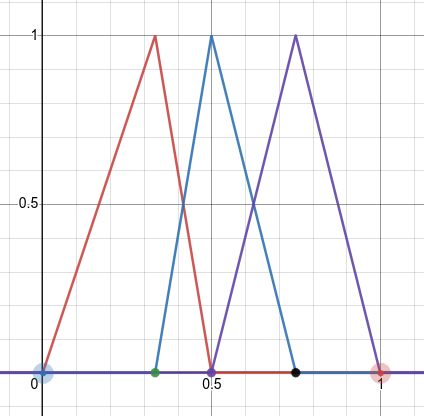
\includegraphics[width=0.7\textwidth]{img/phis}
  \end{center}
  Como buscamos una solución dentro del mismo
  $V_h=\<\phi_1,\phi_2,\phi_3\>$, tenemos
  \begin{equation}
    u_h = \sum_{j=1}^{n}u_j\phi_j
  ,\end{equation}
  y, para resolver $a(u_h,v)=(f,v)$, basta resolver las ecuaciones
  \begin{equation}
    \left\{
      \begin{aligned}
        \sum_{j=1}^{n}u_j a(\phi_j,\phi_1) = (f,\phi_1)
        \\
        \sum_{j=1}^{n}u_j a(\phi_j,\phi_2) = (f,\phi_2)
        \\
        \sum_{j=1}^{n}u_j a(\phi_j,\phi_3) = (f,\phi_3)
      \end{aligned}
    \right.
  \end{equation}
  i.e. la ecuación matricial
  \begin{equation}
    \begin{bmatrix}
      a(\phi_1,\phi_1)
      &a(\phi_2,\phi_1)
      &a(\phi_3,\phi_1)
      \\
      a(\phi_1,\phi_2)
      &a(\phi_2,\phi_2)
      &a(\phi_3,\phi_2)
      \\
      a(\phi_1,\phi_3)
      &a(\phi_2,\phi_3)
      &a(\phi_3,\phi_3)
    \end{bmatrix}
    \begin{bmatrix}
      u_1 \\ u_2 \\ u_3
    \end{bmatrix}
    =
    \begin{bmatrix}
      (f,\phi_1) \\ (f,\phi_2) \\ (f,\phi_3)
    \end{bmatrix}.
  \end{equation}
  Calculemos la matríz de la izquierda. Dado que
  \begin{equation}
    \phi_i(x)
    =
    \begin{cases}
      \frac{x-x_{i-1}}{h_{i-1}} & x\in[x_{i-1},x_i] \\
      \frac{x_{i+1}-x}{h_i} & x\in[x_i,x_{i+1}] \\
      0 & \text{en otro caso},
    \end{cases}
  ,\end{equation}
  tenemos
  \begin{equation}
    \phi_i'(x)
    =
    \begin{cases}
      \frac{1}{h_{i-1}} & x\in[x_{i-1},x_i] \\
      -\frac{1}{h_i} & x\in[x_i,x_{i+1}] \\
      0 & \text{en otro caso}.
    \end{cases}
  \end{equation}
  Luego,
  \begin{align}
    a(\phi_i,\phi_i)
    &= \int_0^{1}\phi_1'(x)^{2}\,dx \\
    &= \int_{x_{i-1}}^{x_i}\frac{1}{h_{i-1}^{2}}\,dx
    + \int_{x_{i}}^{x_{i+1}}\frac{1}{h_{i}^{2}}\,dx \\
    &= \frac{1}{h_{i-1}} + \frac{1}{h_{i}}, \quad i=1,2,3;
    \\
    a(\phi_{i},\phi_{i+1})
    &= a(\phi_{i+1},\phi_i) \\
    &= \int_{x_{i}}^{x_{i+1}}-\frac{1}{h_i^{2}}\,dx \\
    &= -\frac{1}{h_i}, \quad i=1,2
  \end{align}
  y $a(\phi_1,\phi_3)=a(\phi_3,\phi_1)=0$.
  Luego,
  \begin{equation}
    \begin{bmatrix}
      a(\phi_1,\phi_1)
      &a(\phi_2,\phi_1)
      &a(\phi_3,\phi_1)
      \\
      a(\phi_1,\phi_2)
      &a(\phi_2,\phi_2)
      &a(\phi_3,\phi_2)
      \\
      a(\phi_1,\phi_3)
      &a(\phi_2,\phi_3)
      &a(\phi_3,\phi_3)
    \end{bmatrix}
    =
    \begin{bmatrix}
      9 &-6 &0 \\
      -6 &10 &-4 \\
      0 &-4 &8
    \end{bmatrix}
  .\end{equation}
  Ahora el vector de la derecha. Tenemos
  \begin{align}
    (f,\phi_i)
      &= \int_{0}^{1}\pi^{2}\sin(\pi x)\phi_i(x)\,dx
    \\
      &= \frac{\pi^{2}}{h_{i-1}}
      \int_{x_{i-1}}^{x_{i}}\sin(\pi x) (x-x_{i-1})\,dx
      +
      \frac{\pi^{2}}{h_i}
      \int_{x_{i}}^{x_{i+1}}\sin(\pi x)(x_{i+1}-x)\,dx
    \\
    &= 
      \frac{1}{h_{i-1}}
      (-\pi h_{i-1}\cos(\pi x_i) - \sin(\pi x_{i-1})+\sin(\pi x_i))
      \\
      &\quad
      +
      \frac{1}{h_{i}}
      (\pi h_i\cos(\pi x_{i})+\sin(\pi x_i) -\sin(\pi x_{i+1}))
      \\
    &= 
      \frac{1}{h_{i-1}}
      (-\sin(\pi x_{i-1})+\sin(\pi x_i))
      \\
      &\quad
      +
      \frac{1}{h_{i}}
      (\sin(\pi x_i) -\sin(\pi x_{i+1}))
  .\end{align}
  Luego,
  \begin{align}
    (f,\phi_1)
      &= 
      \frac{1}{h_{0}}
      (- \sin(\pi x_{0})+\sin(\pi x_1))
      \\
      &\quad
      +
      \frac{1}{h_{1}}
      (\sin(\pi x_1) -\sin(\pi x_{2}))
    \\
      &= 
      \frac{1}{h_{0}} (-\sin(0) + \sin(\pi / 3))
      \\
      &\quad
      +
      \frac{1}{h_{1}}
      (\sin(\pi / 3) -\sin(\pi / 2))
    \\
      &= 
      \frac{1}{h_{0}} \sqrt{3}/2
      +
      \frac{1}{h_{1}} (\sqrt 3 / 2 - 1)
    \\
      &= 3(\sqrt{3}/2) + 6(\sqrt 3 / 2 - 1)
    \\
      &= 3\sqrt{3}/2 + 3\sqrt 3 - 6
    \\
      &= \frac{9\sqrt{3}}{2} - 6
    \\
    (f,\phi_2)
      &= 
      \frac{1}{h_{1}}
      (- \sin(\pi x_{1})+\sin(\pi x_2))
      \\
      &\quad
      +
      \frac{1}{h_{2}}
      (\sin(\pi x_2) -\sin(\pi x_{3}))
    \\
      &= 
      \frac{1}{h_{1}}
      (- \sin(\pi / 3)+\sin(\pi / 2))
      \\
      &\quad
      +
      \frac{1}{h_{2}}
      (\sin(\pi / 2) -\sin(3\pi / 4))
    \\
      &= 
      \frac{1}{h_{1}} (-\sqrt 3 / 2 + 1)
      +
      \frac{1}{h_{2}}
      (1 - \sqrt 2 / 2 )
    \\
      &= 
      6(-\sqrt 3 / 2 + 1)
      +
      4 (1 - \sqrt 2 / 2 )
    \\
      &= -3\sqrt 3 + 6 + 4 - 2\sqrt 2
    \\
      &= 10 -3\sqrt 3 -2\sqrt 2
    \\
    (f,\phi_3)
      &= 
      \frac{1}{h_{2}}
      (- \sin(\pi x_{2})+\sin(\pi x_3))
      \\
      &\quad
      +
      \frac{1}{h_{3}}
      (\sin(\pi x_3) -\sin(\pi x_{4}))
    \\
      &= 
      \frac{1}{h_{2}}
      (- \sin(\pi / 2)+\sin(3\pi / 4))
      \\
      &\quad
      +
      \frac{1}{h_{3}}
      (\sin(3\pi / 4) -\sin(\pi))
    \\
      &= 
      \frac{1}{h_{2}}
      (- 1+ \sqrt 2 / 2)
      +
      \frac{1}{h_{3}}
      (\sqrt 2 / 2 )
    \\
      &= 
      4
      (- 1+ \sqrt 2 / 2)
      +
      4
      (\sqrt 2 / 2 )
    \\
      &= 4\sqrt 2 - 4
  ,\end{align}
  Así, el sistema que hay que resolver es
  \begin{equation}
    \begin{bmatrix}
      9 &-6 &0 \\
      -6 &10 &-4 \\
      0 &-4 &8
    \end{bmatrix}
    \begin{bmatrix}
      u_1 \\ u_2 \\ u_3
    \end{bmatrix}
    =
    \begin{bmatrix}
      9\sqrt{3} / 2 - 6 \\
      10 -3\sqrt 3 -2\sqrt 2 \\
      4\sqrt 2 - 4
    \end{bmatrix}.
  \end{equation}
  La solución es
  \begin{equation}
    \begin{bmatrix}
      u_1 \\ u_2 \\ u_3
    \end{bmatrix}
    =
    \begin{bmatrix}
      \sqrt 3 / 2 \\
      1 \\
      \sqrt 2 / 2
    \end{bmatrix}
  .\end{equation}
  Entonces
  \begin{equation}
    u_h
    =
    \frac{\sqrt 3}{2}\phi_1
    + \phi_2
    + \frac{\sqrt 2}{2}\phi_3
  .\end{equation}
  En la siguiente gráfica se muestran la solución real
  $u(x)=\sin(\pi x)$ y la aproximación obtenida:
  \begin{center}
  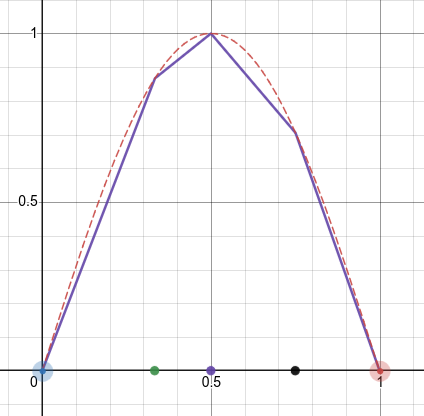
\includegraphics[width=0.7\textwidth]{img/sol_vs_aprox}
  \end{center}
\end{sol}

\begin{exercise}
  Considere el problema
  \begin{equation}
    \left\{
      \begin{aligned}
        & u_t + a u_x = 0,
        \\
        & u(x,0) = f(x),
      \end{aligned}
    \right.
  \end{equation}
  donde $a>0$ es una constante. Calcule el error de truncamiento local
  para los métodos FTCS y upwind.
\end{exercise}
\begin{sol}
  El método FTCS nos da el esquema
  \begin{equation}
    u_j^{k+1} = u_j^k - a\Delta t \frac{u_{j+1}^k-u_{j-1}^k}{2h}
  .\end{equation}
  Los métodos son
  \begin{align}
    &\frac{u(x_j,t_{k+1}) - u(x_{j},t_k)}{\Delta t}
    \\
      &=
      \frac
      {
        u(x_j,t_k)
        +\Delta tu_t(x_j,t_k)
        +(\Delta t)^{2}/2 u_{tt}(x_j,t_k)
        + O((\Delta t)^{3})
        - u(x_{j},t_k)
      }
      {\Delta t}
      \\
      &=
        u_t(x_j,t_k)
        +\frac{\Delta t}{2} u_{tt}(x_j,t_k)
        + O((\Delta t)^{2})
  \end{align}
  y
  \begin{align}
    &\frac{u(x_{j+1},t_k)-u(x_{j-1},t_k)}{2h} \\
    &=
    \frac{
      u(x_j,t_k)
      + hu_x(x_j,t_k)
      +\frac{h^{2}}{2}u_{xx}(x_j,t_k)
      +\frac{h^{3}}{6}u_{xxx}(x_j,t_k)
      +O(h^{4})
      }{2h} \\
      &\quad - \frac{
      u(x_{j},t_k)
      - h u_{x}(x_{j},t_k)
      +\frac{h^{2}}{2} u_{xx}(x_j,t_k)
      - \frac{h^{3}}{6}u_{xxx}(x_j,t_k)
      +O(h^{4})
      }{2h}
  .\end{align}
  Luego, si $u(x,t)$ es la solución exacta, tenemos
  \begin{align}
    &\frac{u(x_j,t_{k+1}) - u(x_{j},t_k)}{\Delta t}
    + a \frac{u(x_{j+1},t_k)-u(x_{j-1},t_k)}{2h}
    \\
      &=
        u_t(x_j,t_k)
        +\frac{\Delta t}{2} u_{tt}(x_j,t_k)
        + O((\Delta t)^{2})
        \\
      &\quad
      + au_x(x_j,t_k) +a\frac{h^{2}}{6}u_{xxx}(x_j,t_k)
      +O(h^{3})
    \\
      &=
        \frac{\Delta t}{2} u_{tt}(x_j,t_k)
        + a \frac{h^{2}}{6}u_{xxx}(x_j,t_k)
        + O((\Delta t)^{2},h^{3})
  .\end{align}
  

  
\end{sol}

\end{document}
